\subsection{识读要点}
\subsubsection{视图中线框和图形的理解}
一、视图中的每个线框,通常表示的是物体上一个表面(平面、曲面或平面和曲面相切)的投影。图\ref{fig:kantu8}中,线框A和E代表一个平面,线框F代表一个曲面,线框E代表平面和典相切。

二、视图中的相邻线框,表示物体上不同位置的两个表面。两个表面或是上下、左右、前后的位置关系,或者是两表面相交。图\ref{fig:kantu8}中,A、D两个面,A面在上,B面在下;A、D两个面,A面在右,D面在左。

\begin{figure}[htbp]
\centering
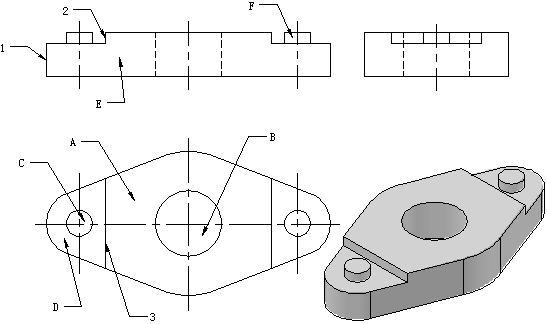
\includegraphics[scale=0.9]{kantu8.png}
\caption{线框和图形的含义}\label{fig:kantu8}
\end{figure}


三、视图中大线框套小线框,表示物体龙须面上凸出或凹进的关系。图\ref{fig:kantu8}中,C、D两个面,C为凸出;A、B两个面,B为凹进。

四、视图中的第一条线,可能是立体表面有积聚性表面的投影,如图\ref{fig:kantu8}中的线2;也可能是两平面的投影,如图\ref{fig:kantu8}中的线3;也可能是曲面转向轮廓线的投影,如图\ref{fig:kantu8}中的线1。
\subsubsection{联系多个视图进行识读}
在缺少尺寸瓢的情况下,一个视图是不能够确定物体的形状的。因为一个视图只能够表达两个方向的尺寸,一般不能够确切地表达出物体的三维空间形状。如图\ref{fig:kantu9}所示,如果仅仅只用主视图难以准确表达出物体的三维形状。根据俯视图的不同,物体的底板可能是倒角、凸字形和凹字形。因此,看图不能仅看一个或两个视图,而要把三个视图联系起来进行分析,才能够确定物体的形状。

\begin{figure}[htbp]
\centering
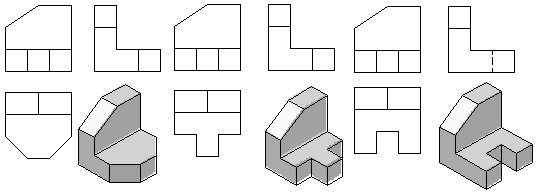
\includegraphics[scale=0.9]{kantu9.png}
\caption{一个视图不能确切地表达物体的形状}\label{fig:kantu9}
\end{figure}

如果视图选择不当,即使有两个视图也不能够准确地表达出物体的三维形状。如图\ref{fig:kantu9}所示,如果采用主视图和左视图就不能够清楚地表达出物体的形状。


\subsubsection{确定主特征视图}
特征视图是能够充分反映物体形状或相互位置特征的视图。特征视图通常分类形状特征视图和位置特征视图。形状特征图是能够充分反映物体形状特征的视图。图\ref{fig:kantu10}的主视图为形状特征视图,\ref{fig:kantu11}的俯视图为形状特征视图,它们都充分反映了特征的形状特征
\begin{figure}[htbp]
\centering
\subfloat[主视图为形状特征视图]{\label{fig:kantu10}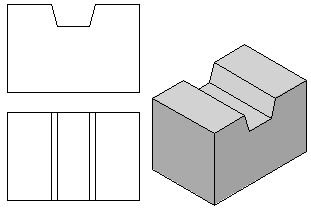
\includegraphics[scale=0.7]{kantu10.png}}\hspace{30pt}
\subfloat[俯视图为形状特征视图]{\label{fig:kantu11}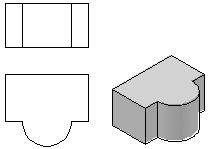
\includegraphics[scale=1]{kantu11.png}}
\caption{形状特征视图}
\end{figure}

位置特征图是能够充分反映相互位置特征的视图。图\ref{fig:kantu12}和\ref{fig:kantu13}所示的主视图是物体的形状特征图,但仅依靠主视图和俯视图不能够确定出1和2两个线框所代表的形状的具体位置。它们的左视图则清楚地反映方孔和圆柱的具体位置关系。
\begin{figure}[htbp]
\centering
\subfloat[]{\label{fig:kantu12}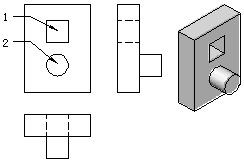
\includegraphics[scale=0.9]{kantu12.png}}\hspace{30pt}
\subfloat[]{\label{fig:kantu13}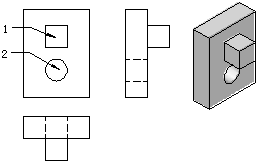
\includegraphics[scale=0.9]{kantu13.png}}
\caption{位置特征视图}
\end{figure}
\subsubsection{注意反映形体联接关系的图线}
形体之间的联接关系的变化,会导致视图中的图线产生相应的变化。图\ref{fig:kantu14}所示,三角形肋板与底板的连接是实线,说明它们的前面不是位于同一平面的错位关系,由俯视图可知三角形肋板位于底板中间。图\ref{fig:fati15}的中间是虚线连接,三角形肋板与底板的前面是位于同一个平面的,根据俯视图可以确定三角形肋板有两块,一块位于前面,另一块位于后面。
\begin{figure}[htbp]
\centering
\subfloat[]{\label{fig:kantu14}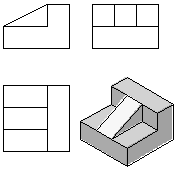
\includegraphics[scale=0.9]{kantu14.png}}\hspace{30pt}
\subfloat[]{\label{fig:kantu15}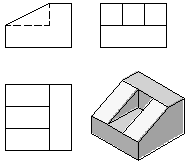
\includegraphics[scale=0.9]{kantu15.png}}
\caption{形体之间的表面联接关系}
\end{figure}
\endinput